\documentclass[12pt, letterpaper] {article}

\parindent=5mm
\usepackage[spanish]{babel}

\usepackage{amssymb}
\usepackage{amsmath} 
\usepackage{amsfonts}

\usepackage[numbers,sort&compress]{natbib}
\usepackage{graphicx}

\usepackage{url}
\usepackage{hyperref}

\usepackage[top=25mm, bottom=20mm, left=1.5cm, right=1.5cm]{geometry}
\setlength{\parskip}{2mm}
\setlength{\parindent}{1pt}

\usepackage{listings}

\usepackage{float}

\usepackage[utf8]{inputenc}
\usepackage{graphicx} 
\usepackage{subfigure} 

\usepackage{color}
\usepackage{multirow}

\definecolor{dkgreen}{rgb}{0,0.6,0}
\definecolor{gray}{rgb}{0.5,0.5,0.5}
\definecolor{mauve}{rgb}{0.58,0,0.82}

\usepackage[table,xcdraw]{xcolor}

\usepackage{color}
\usepackage{listings}
\lstset{ %
  language=R,                     % the language of the code
  basicstyle=\footnotesize,       % the size of the fonts that are used for the code
  numbers=left,                   % where to put the line-numbers
  numberstyle=\tiny\color{gray},  % the style that is used for the line-numbers
  stepnumber=1,                   % the step between two line-numbers. If it's 1, each line
                                  % will be numbered
  numbersep=5pt,                  % how far the line-numbers are from the code
  backgroundcolor=\color{white},  % choose the background color. You must add \usepackage{color}
  showspaces=false,               % show spaces adding particular underscores
  showstringspaces=false,         % underline spaces within strings
  showtabs=false,                 % show tabs within strings adding particular underscores
  frame=single,                   % adds a frame around the code
  rulecolor=\color{black},        % if not set, the frame-color may be changed on line-breaks within not-black text (e.g. commens (green here))
  tabsize=2,                      % sets default tabsize to 2 spaces
  captionpos=b,                   % sets the caption-position to bottom
  breaklines=true,                % sets automatic line breaking
  breakatwhitespace=false,        % sets if automatic breaks should only happen at whitespace
  title=\lstname,                 % show the filename of files included with \lstinputlisting;
                                  % also try caption instead of title
  keywordstyle=\color{blue},      % keyword style
  commentstyle=\color{dkgreen},   % comment style
  stringstyle=\color{mauve},      % string literal style
  escapeinside={\%*}{*)},         % if you want to add a comment within your code
  morekeywords={*,...}            % if you want to add more keywords to the set
} 


\author{Ricardo Rosas Macías}

\title{Práctica 8: modelo de urnas}

\date{\today}

\begin{document}

\maketitle


\section{Introducción}
El modelo de urnas arriba los fenómenos coalescencia y fragmentación, de modo en que une las partículas que se encuentran divididas en dos o más pedazos más pequeños; siempre siendo un entero. Este experimento tiene una reacción parecida a los agentes coagulantes en donde las partículas más pequeñas se agrupan para formar una más grande y así poder ser separada de una manera más fácil. 

 \section{Objetivo}
Se realizó cambios en el c\'odigo proporcionado en la p\'agina web \cite{elisawebUrna}, de manera que al paralelilzar se vuelva más eficiente realizando varias tareas al mismo tiempo y así reducir el tiempo total de la ejecución del código, asimismo se busca visualizar el cambio al generar repeticiones del experimento.

 
 \subsection{Descripción}
 
La finalidad del experimento es \cite{elisawebUrna}:
\begin{quotation}
 ``Paralelizar tanto como resulte eficientemente posible en esta simulación y medir cuánto tiempo se logra ahorrar, de igual manera evaluar si el ahorro es estadísticamente significativo para diferentes combinaciones de partículas y cúmulos.

Para el primer reto, se determinó en cuál momento (en términos del número de iteraciones de la simulación) la fracción de éstas alcance un máximo. Calcula y gráfica esta fracción a lo largo de la simulación. Realiza 30 réplicas para determinar si el número de paso en el cual se alcanza el máximo tiene un comportamiento sistemático.''
\end{quotation}

\section{Resultados y conclusiones}

En base al trabajo anteriormente reportado \cite{Pr8Js}, se realizó el código que se muestra en la parte inferior. En las primeras líneas del c\'odigo se defini\'o los par\'ametros de experimentaci\'on con las cuales se trabajar\'ia, asimismo se ejecutó una paralelización para que el experimento fuera más eficiente. Además se realizó una comparación de la ejecución del experimento en donde se ponderaron diferentes valores para las partículas que están representadas como ``k'' y para los cúmulos definidos con la variante ``n'', como se muestra en el cuadro \ref{PondEx}.

\begin{table}[H]
\caption{Combinación de valores de variables del experimento}\label{PondEx}
\centering
\begin{tabular}{|l|l|l|}
\hline
\rowcolor[HTML]{EFEFEF} 
\multicolumn{1}{|c|}{\cellcolor[HTML]{EFEFEF}{\color[HTML]{333333} Nombre}} & \multicolumn{1}{c|}{\cellcolor[HTML]{EFEFEF} n } & \multicolumn{1}{c|}{\cellcolor[HTML]{EFEFEF} k} \\ \hline
\rowcolor[HTML]{ECF4FF} 
{\color[HTML]{333333} C1}                                        & {\color[HTML]{333333} 100}                                  & {\color[HTML]{333333} 10000}                             \\ \hline
\rowcolor[HTML]{ECF4FF} 
{\color[HTML]{333333} C2}                                        & {\color[HTML]{333333} 1000}                                 & {\color[HTML]{333333} 100000}                            \\ \hline
\rowcolor[HTML]{ECF4FF} 
{\color[HTML]{333333} C3}                                        & {\color[HTML]{333333} 10000}                                & {\color[HTML]{333333} 1000000}                           \\ \hline
\end{tabular}
\end{table}

\begin{lstlisting}[language=R]
k <- c(100, 1000, 10000)
n <- c(10000, 100000, 1000000)

suppressMessages(library(doParallel))
registerDoParallel(clust)
cluster <- makeCluster(detectCores()-1) 
clusterExport(cluster, "romperse") 
clusterExport(cluster, "rotura") 
clusterExport(cluster, "funromperse") 
clusterExport(cluster, "c") 
clusterExport(cluster, "d") 
clusterExport(cluster, "assert") 
clusterExport(cluster, "fununirse") 
clusterExport(cluster, "union") 
clusterExport(cluster, "unirse") 
TimeF <- NULL
TimeF <- microbenchmark(exect2 = {
  originales <- rnorm(k)
  cumulos <- originales - min(originales) + 1
  cumulos <- round(n * cumulos / sum(cumulos))
  assert(min(cumulos) > 0)
  diferencia <- n - sum(cumulos)
  if (diferencia > 0) {
    for (i in 1:diferencia) {
      p <- sample(1:k, 1)
      cumulos[p] <- cumulos[p] + 1
    }
  } else if (diferencia < 0) {
    
    for (i in 1:-diferencia) {
      p <- sample(1:k, 1)
      if (cumulos[p] > 1) {
        cumulos[p] <- cumulos[p] - 1
      }
    }
    
  }
  for (paso in 1:duracion) {
    assert(sum(cumulos) == n)
    cumulos <- integer()
  
    for (i in 1:dim(freq)[1]) { # fase de rotura
      urna <- freq[i,]
      if (urna$tam > 1) { # no tiene caso romper si no se puede
        cumulos <- c(cumulos, romperse(urna$tam, urna$num))
      } else {
        cumulos <- c(cumulos, rep(1, urna$num))
      }
    }
  }
}, times = 10, unit = "s")
stopCluster(clust)
print(Ptime)
print(TimeF)
tiempos <- rbind(Ptime, TimeF)
tiempos <- data.frame(tiempos)
tiempos$time <- tiempos$time/10**9
tiempos$expr <- as.factor(tiempos$expr)
\end{lstlisting}

Como se menciona en el apartado anterior, para observar cambios significativos en el tiempo del experimento se vario los valores de las partículas y cúmulos respectivamente, de manera que los datos proporcionados se muestran en la gráfica \ref{GF}, en donde se puede observar claramente que los tiempos al parelizar son mejores a comparación de la ejecución normal. Por lo tanto es un factor determinante para optar por el uso de dicha función.

\begin{figure}[H]
\centering
\subfigure[C1]{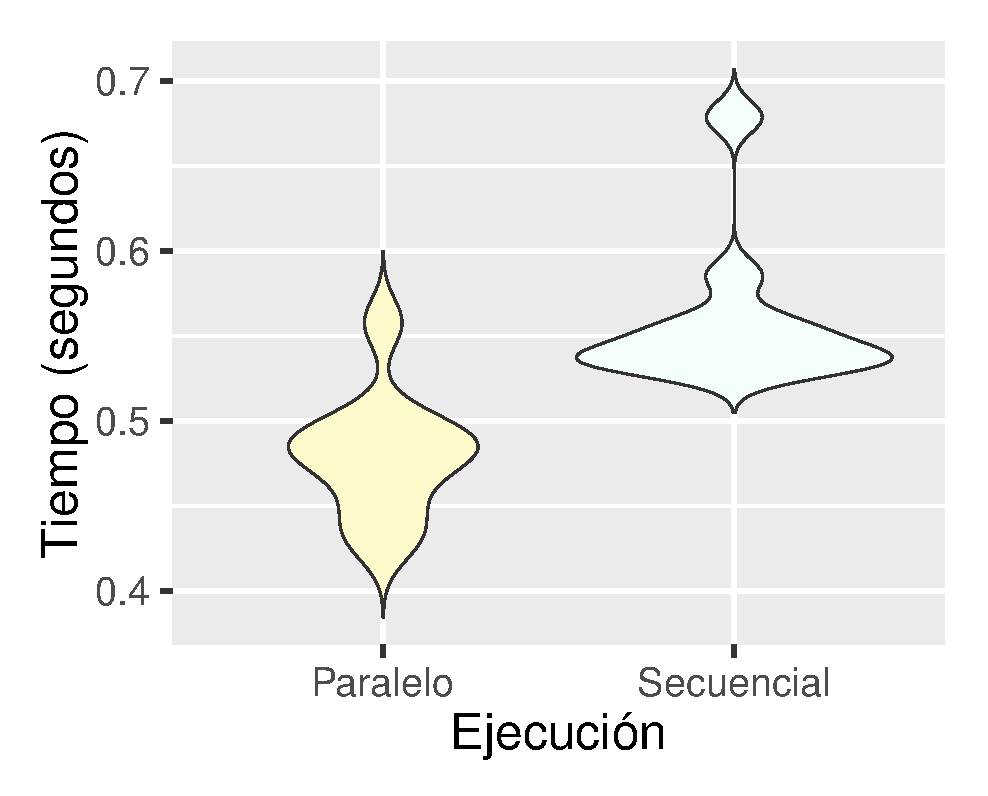
\includegraphics[width=60mm]{./E1}}\vspace{1mm}
\subfigure[C2]{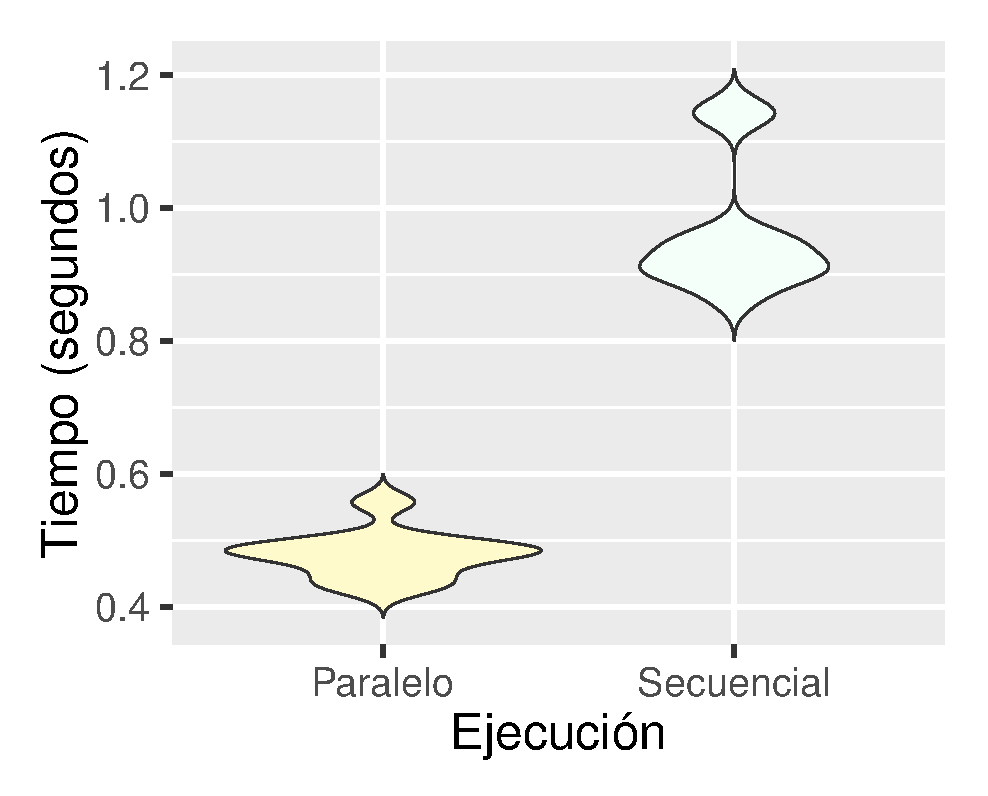
\includegraphics[width=60mm]{./E2}}
\subfigure[C3]{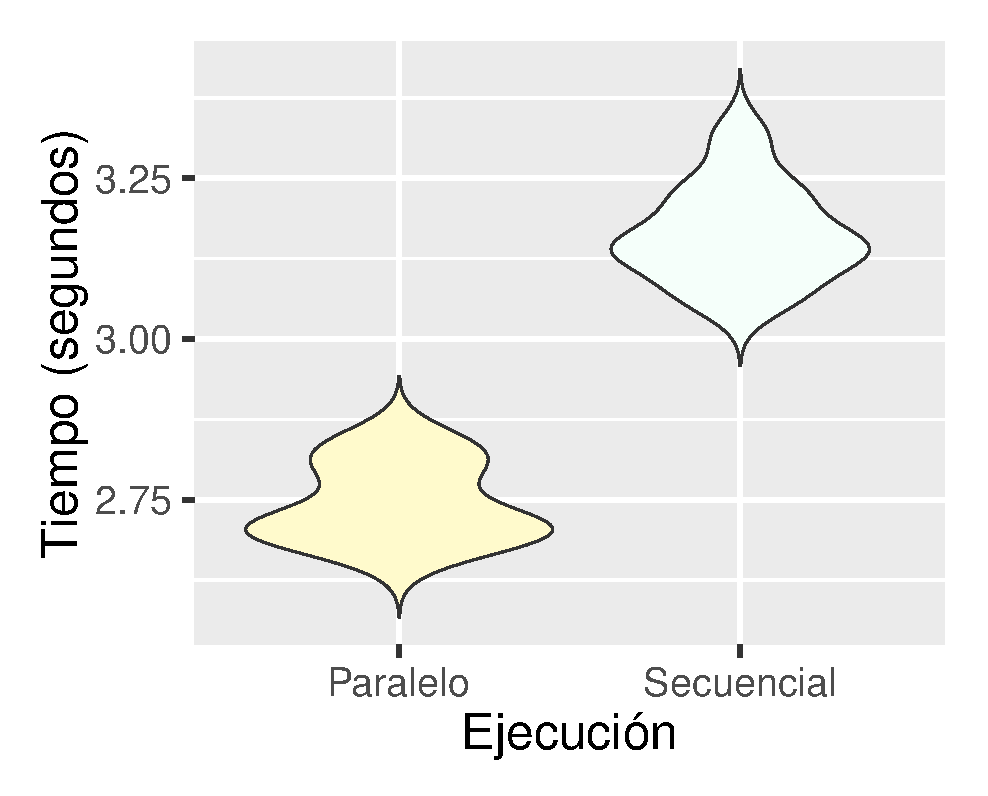
\includegraphics[width=60mm]{./E3}}
\caption{Tiempo del experimento}\label{GF}
\end{figure}


\subsection{Reto 1}

Para el primer reto se creó un código en el cual se pueda replicar por 30 veces, como se muestra en las líneas de la parte inferior. Asimismo se usaron las combinaciones anteriores para determinar si el experimento tiene un comportamiento sistemático.

\begin{lstlisting}[language=R]
k <- c(100, 1000, 10000)
n <- c(10000, 100000, 1000000)

funromperse <- function(i){ 
  return(as.vector(romperse(as.numeric(freq[i,][1]), as.numeric(freq[i,][2])))) 
} 
fununirse <- function(i){ 
  return(unirse(as.numeric(freq[i,][1]), as.numeric(freq[i,][2]))) 
} 

cluster <- makeCluster(detectCores()-1) 
clusterExport(cluster,"romperse") 
clusterExport(cluster,"rotura") 
clusterExport(cluster,"funromperse") 
clusterExport(cluster,"c") 
clusterExport(cluster,"d") 
clusterExport(cluster,"assert") 
clusterExport(cluster,"fununirse") 
clusterExport(cluster,"union") 


vartime <- data.frame()
for (repeticiones in 1:30) {
  tiempoinicial <- Sys.time()
  for (paso in 1:duracion) { 
    assert(sum(cumulos) == n) 
    cumulos <- integer() 
    clusterExport(cluster, "freq") 
    cumulos <- as.vector(parSapply(cluster, 1:(dim(freq)[1]), funromperse)) 
    a <- c() 
    for(i in 1:length(cumulos)){ 
      a <-c(a, cumulos[[i]]) 
    } 
    cumulos <- a 

 clusterExport(cluster, "freq") 
    cumulos <- as.vector(parSapply(cluster, 1:(dim(freq)[1]), fununirse)) 
    a <- c() 
    for(i in 1:length(cumulos)){ 
      a <-c(a, cumulos[[i]]) 
    } 
    cumulos <- a 
\end{lstlisting}

En la figura \ref{ItSi} se muestra la variación del máximo de las repeticiones de la ejecución, las cuales demuestran una tendencia a disminuir la variación en el tiempo de ejecución de las replicas, debido al incremento en los valores de la combinación de partículas y cúmulos. De manera que se puede determinar que el experimento tiene un comportamiento sistemático. 

\begin{figure}[H]
\centering
\subfigure[Tiempo de C1]{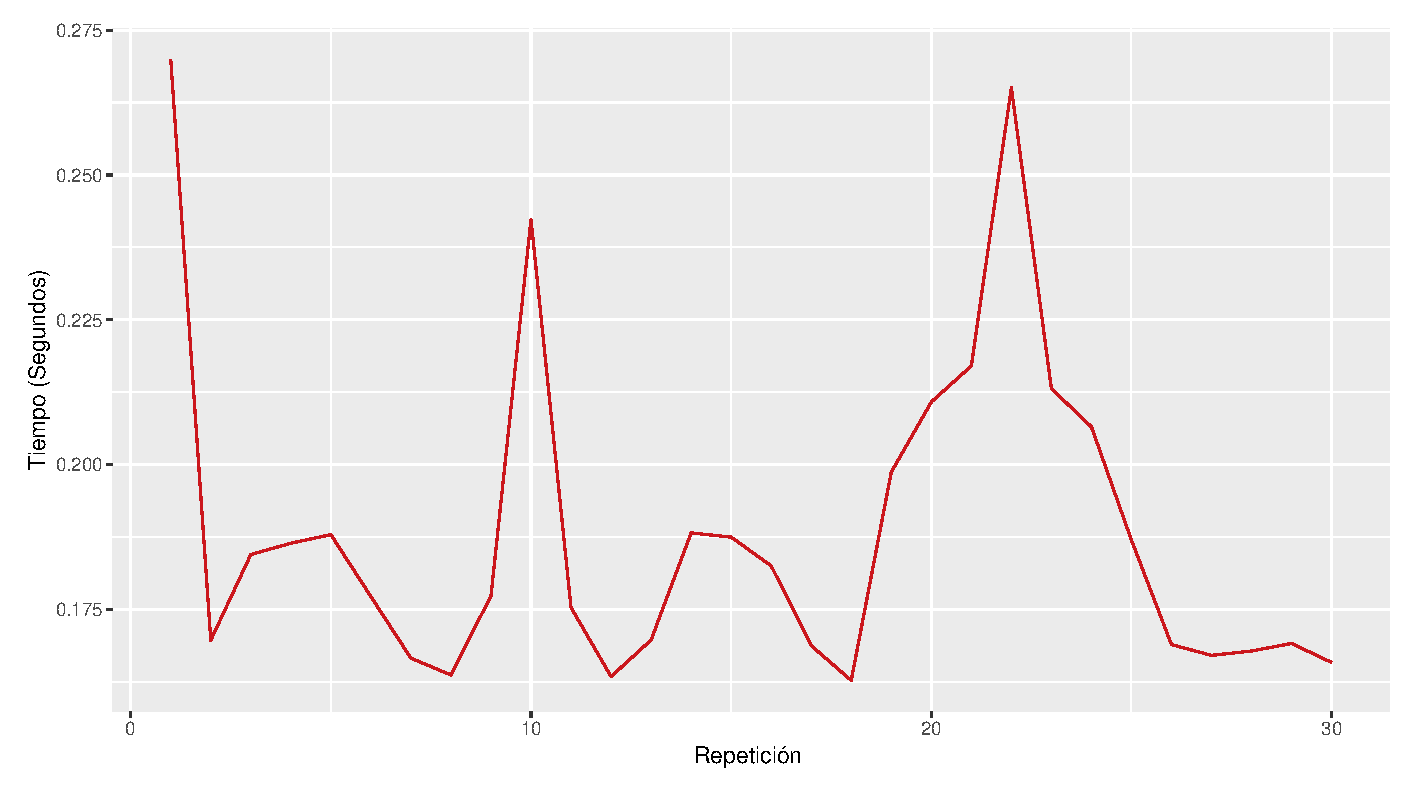
\includegraphics[width=90mm]{./Time1}}\vspace{1mm}
\subfigure[Tiempo de C2]{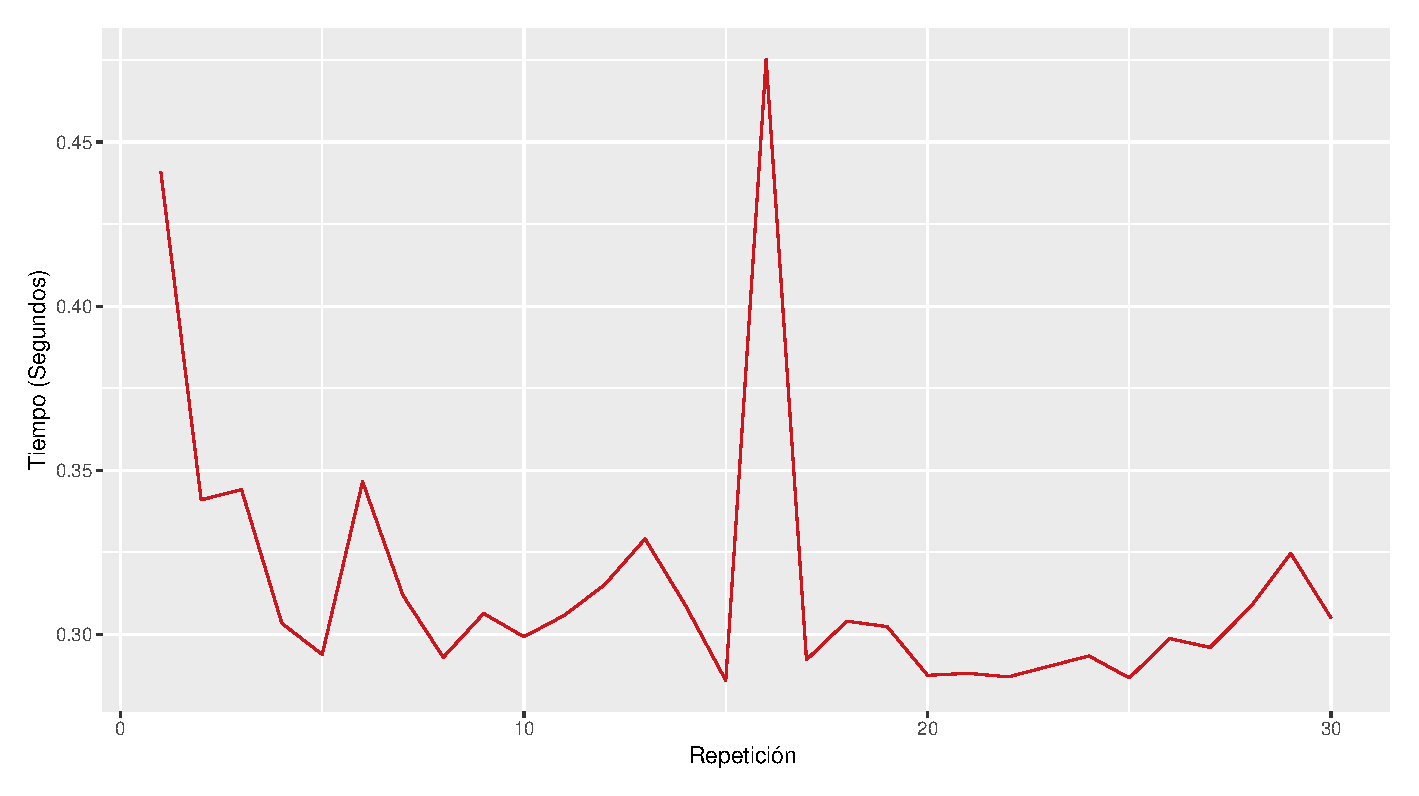
\includegraphics[width=90mm]{./Time2}}
\subfigure[Tiempo de C3]{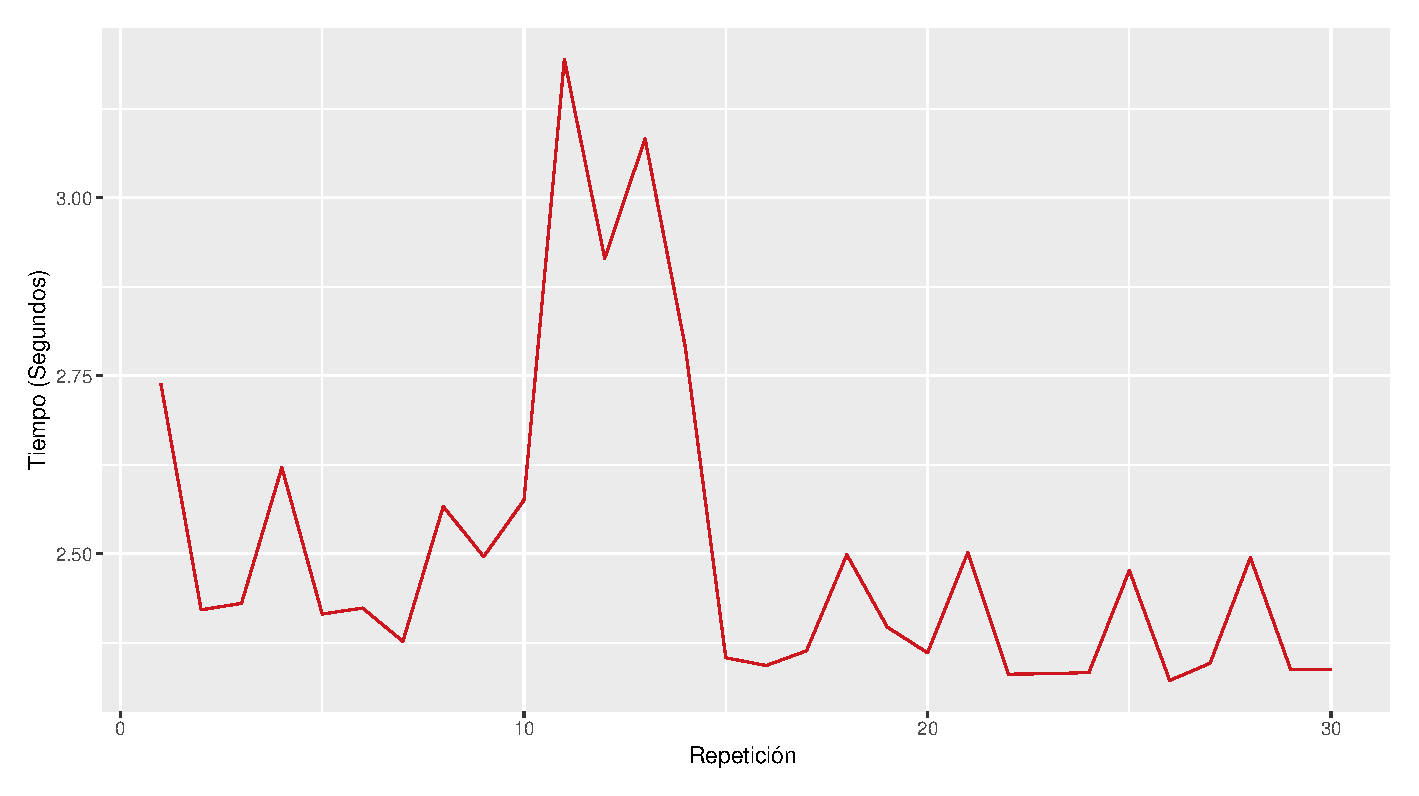
\includegraphics[width=90mm]{./Time3}}
\caption{Iteraciones de la simulación}\label{ItSi}
\end{figure}


\bibliographystyle{plainnat}

\bibliography{BiblioHWP8}

\end{document}